\documentclass[dvipdfmx,cjk,xcolor=dvipsnames,envcountsect,notheorems,12pt]{beamer}
% * 16:9 のスライドを作るときは、aspectratio=169 を documentclass のオプションに追加する
% * 印刷用の配布資料を作るときは handout を documentclass のオプションに追加する
%   (overlay が全て一つのスライドに出力される)

\usepackage{pxjahyper}% しおりの文字化け対策 (なくても良い)
\usepackage{amsmath,amssymb,amsfonts,amsthm,ascmac,cases,bm,pifont}
\usepackage{graphicx}
\usepackage[thicklines]{cancel}
\usepackage{url}
\usepackage{newtxmath}
\usepackage{bussproofs}

% スライドのテーマ
\usetheme{sumiilab}
% ベースになる色を指定できる
%\usecolortheme[named=Magenta]{structure}
% 数式の文字が細くて見難い時は serif の代わりに bold にしましょう
%\mathversion{bold}

%% ===============================================
%% スライドの表紙および PDF に表示される情報
%% ===============================================

%% 発表会の名前とか(省略可)
\session{ML勉強会}
%% スライドのタイトル
\title{MLでAtCoderに参加した話}
%% 必要ならば、サブタイトルも
%\subtitle{}
%% 発表者のお名前
\author{@fetburner}
%% 発表者の所属([] 内は短い名前)
%\institute[東北大学 住井・松田研]{工学部 電気情報物理工学科\\住井・松田研究室}% 学部生
%\institute[東北大学 住井・松田研]{大学院情報科学研究科\\住井・松田研究室}% 院生
%% 発表する日
\date{2017年7月22日}

%% ===============================================
%% 自動挿入される目次ページの設定(削除しても可)
%% ===============================================

% section の先頭に自動挿入される目次ページ(削除すると、表示されなくなる)
\AtBeginSection[]{
\begin{frame}
  \frametitle{アウトライン}
  \tableofcontents[sectionstyle=show/shaded,subsectionstyle=show/show/hide]
\end{frame}}
% subsection の先頭に自動挿入される目次ページ(削除すると、表示されなくなる)
\AtBeginSubsection[]{
\begin{frame}
  \frametitle{アウトライン}
  \tableofcontents[sectionstyle=show/shaded,subsectionstyle=show/shaded/hide]
\end{frame}}
%% 現在の section 以外を非表示にする場合は以下のようにする

%% \AtBeginSection[]{
%% \begin{frame}
%%   \frametitle{アウトライン}
%%   \tableofcontents[sectionstyle=show/hide,subsectionstyle=show/show/hide]
%% \end{frame}}
%% \AtBeginSubsection[]{
%% \begin{frame}
%%   \frametitle{アウトライン}
%%   \tableofcontents[sectionstyle=show/hide,subsectionstyle=show/shaded/hide]
%% \end{frame}}

%% ===============================================
%% 定理環境の設定
%% ===============================================

\setbeamertemplate{theorems}[numbered]% 定理環境に番号を付ける
\theoremstyle{definition}
\newtheorem{definition}{定義}
\newtheorem{axiom}{公理}
\newtheorem{theorem}{定理}
\newtheorem{lemma}{補題}
\newtheorem{corollary}{系}
\newtheorem{proposition}{命題}

%% ===============================================
%% ソースコードの設定
%% ===============================================

\usepackage{listings,jlisting}
%\usepackage[scale=0.9]{DejaVuSansMono}

\definecolor{DarkGreen}{rgb}{0,0.5,0}
% プログラミング言語と表示するフォント等の設定
\lstset{
  language={[Objective]Caml},% プログラミング言語
  basicstyle={\ttfamily\small},% ソースコードのテキストのスタイル
  keywordstyle={\bfseries},% 予約語等のキーワードのスタイル
  commentstyle={},% コメントのスタイル
  stringstyle={},% 文字列のスタイル
  frame=trlb,% ソースコードの枠線の設定 (none だと非表示)
  numbers=none,% 行番号の表示 (left だと左に表示)
  numberstyle={},% 行番号のスタイル
  xleftmargin=5pt,% 左余白
  xrightmargin=5pt,% 右余白
  keepspaces=true,% 空白を表示する
  mathescape,% $ で囲った部分を数式として表示する ($ がソースコード中で使えなくなるので注意)
  % 手動強調表示の設定
  moredelim=[is][\itshape]{@/}{/@},
  moredelim=[is][\color{red}]{@r\{}{\}@},
  moredelim=[is][\color{blue}]{@b\{}{\}@},
  moredelim=[is][\color{DarkGreen}]{@g\{}{\}@},
}

\newcommand{\keyword}[1]{\mathbf{#1}}
\newcommand{\LET}{\keyword{let}}
\newcommand{\IN}{\keyword{in}}

%% ===============================================
%% 本文
%% ===============================================
\begin{document}
\frame[plain]{\titlepage}% タイトルページ

\begin{frame}
	\frametitle{自己紹介}
	\begin{itemize}
		\item 水野雅之
		\item Twitter:@fetburner
		\item Coqでメタ定理の形式化やってるM2
			\begin{itemize}
				\item 日常生活でCoqしか書かなさすぎてヤバいので競プロでMLのリハビリ
			\end{itemize}
	\end{itemize}
	\begin{figure}[hb]
		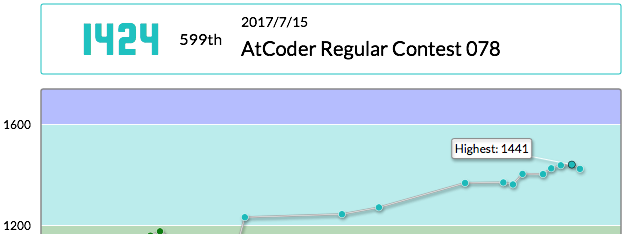
\includegraphics[width=80mm]{./Rating.png}
	\end{figure}
	\begin{center}
		水色コーダーですが,宜しければしばしお付き合いを
	\end{center}
\end{frame}

\begin{frame}
	\frametitle{Q. なぜAtCoder?}
	\begin{itemize}
		\item A. 初期の頃からOCamlをサポートしていたから
			\begin{itemize}
				\item ABC 001 (2013年10月)の頃には既にしてた
				\item 現在処理系はOCaml 4.02.3と比較的新しい
					\begin{itemize}
						\item 昔はOCaml 3.12.1でつらかった
					\end{itemize}
				\item ocamloptでコンパイルするので,定数倍でTLEしない
					\begin{itemize}
						\item 昔はocamlcなので(ry
					\end{itemize}
				\item intが63bitなのでオーバーフロー知らず
			\end{itemize}
		\item 現在ではSML (MLton)もサポート
			\begin{itemize}
				\item これも定数倍でTLEしにくい
				\item intが31bitなので最悪
			\end{itemize}
	\end{itemize}
\end{frame}

\section{簡単な問題と入出力テンプレ}

\begin{frame}
	\frametitle{(早速ですが)問題例1: 単純な入出力}
	\begin{block}{}
		{\Large ``高橋君はデータの加工が行いたいです。
		整数$a,b,c$と、文字列$s$が与えられます。
		整数$a+b+c$と、文字列$s$を並べて表示しなさい。''}
		\begin{flushright}
			--- practice contest A - はじめてのあっとこーだー
		\end{flushright}
	\end{block}
	\vfill
	{\large 競プロではこの問題と同じように,標準入力から\\受け取った値を加工して標準出力に流すプログラムが求められる場合が多い}
\end{frame}

\begin{frame}[fragile]
	\frametitle{OCamlによる解答例}
	\begin{lstlisting}
let () =
  let a = @r{Scanf.scanf}@ "%d\n" (fun a -> a) in
  let b, c = @r{Scanf.scanf}@ "%d %d\n"
    (fun b c -> b, c) in
  let s = @r{Scanf.scanf}@ "%s\n" (fun s -> s) in
  @r{Printf.printf}@ "%d %s\n" (a + b + c) s
\end{lstlisting}
	\begin{itemize}
		\item 入力には\text{Scanf.scanf}を使おう
			\begin{itemize}
				\item OCamlにもあります
				\item 空白や改行の読み飛ばしが容易
			\end{itemize}
		\item 出力には\text{Printf.printf}を使おう
			\begin{itemize}
				\item OCamlにも(ry
				\item フォーマットに沿った出力がしやすい
			\end{itemize}
	\end{itemize}
\end{frame}

\begin{frame}[fragile]
	\frametitle{SMLによる解答例}
	\begin{lstlisting}
fun readInt () =
  @r{TextIO.scanStream (Int.scan StringCvt.DEC)}@
    TextIO.stdIn
val SOME a = readInt ()
val SOME b = readInt ()
val SOME c = readInt ()
(* skip newline *)
val _ = TextIO.inputLine TextIO.stdIn
val SOME s = TextIO.inputLine TextIO.stdIn
val () = print
  (Int.toString (a + b + c) ^ " " ^ s)
\end{lstlisting}
	\begin{itemize}
		\item 数値の入力には\text{StringCvt}を用いる
			\begin{itemize}
				\item Basis Libraryには\text{printf}も\text{scanf}もない(絶望)
			\end{itemize}
	\end{itemize}
\end{frame}

\begin{frame}
	\frametitle{問題例2: 任意個の入出力}
	\begin{block}{}
		{\large ``長さ$n$の数列$a_1,\cdots,a_n$が与えられます。空の数列$b$に対して、以下の操作を$n$回行うことを考えます。

		\smallskip

		$i$回目には

		\smallskip

		1. 数列の$i$番目の要素$a_i$を$b$の末尾に追加する。\\
		2. $b$を逆向きに並び替える。\\

		\smallskip

		この操作をしてできる数列$b$を求めて下さい。''}
		\begin{flushright}
			--- ARC 077 C - pushpush
		\end{flushright}
	\end{block}
\end{frame}

\begin{frame}[fragile]
	\frametitle{OCamlによる解答例}
	\begin{lstlisting}
let () =
  let n = Scanf.scanf "%d\n" (fun n -> n) in
  let as_ = @r{Array.init}@ n (fun _ ->
    Scanf.scanf "%d " (fun a -> a)) in
  @r{Array.fold_left}@ (fun (xs, ys) a ->
    (ys, a :: xs)) ([], []) as_
  |> (fun (xs, ys) -> ys @ List.rev xs)
  |> List.iter (Printf.printf "%d ")
\end{lstlisting}
	\begin{itemize}
		\item 任意個のデータを入力する際には\text{Array.init}が便利
		\item 陽な再帰関数を書く前に\text{fold}で書けないか検討しよう
	\end{itemize}
\end{frame}

\begin{frame}[fragile]
	\frametitle{SMLによる解答例}
	\begin{lstlisting}
val SOME n = readInt ()
val as_=@r{List.tabulate}@(n,fn _=>valOf(readInt()))
val () =
 let val (xs, ys) =
  @r{foldl}@(fn(a,(xs,ys))=>(ys,a::xs))([],[])as_ in
  app(fn x=>print(Int.toString x^" "))(ys@rev xs);
  print "\n"
 end
\end{lstlisting}
	\begin{itemize}
		\item 任意個のデータを入力する際には\text{List.tabulate}が便利
		\item 陽な再帰関数を書く前に\text{fold} (ry
	\end{itemize}
	\begin{flushright}
		構文が重い(半ギレ)
	\end{flushright}
\end{frame}

\section{便利な標準ライブラリ関数の紹介}

\begin{frame}
	\frametitle{\text{List.fold\_left}及び\text{foldl}}
	\begin{itemize}
		\item ライブラリを整備して良し,問題を解いて良し
		\item ABC/ARCのCやAGCのAぐらいまではfoldだけで解ける場合が多い
		\item まずはこれを使いこなしましょう
	\end{itemize}
\end{frame}

\begin{frame}[fragile]
	\frametitle{\text{fold}の例1: 総和}
	\begin{itemize}
		\item ある時は総和を求め
	\begin{lstlisting}
List.fold_left ( + ) 0 xs
\end{lstlisting}
	\vfill
		\item またある時は総乗を求め
	\begin{lstlisting}
List.fold_left ( * ) 1 xs
\end{lstlisting}
	\vfill
		\item 剰余類もなんのその
	\begin{lstlisting}
List.fold_left (fun x y -> x * y mod n) 1
  List.map (fun x -> x mod n) xs
\end{lstlisting}
	\end{itemize}
	\begin{flushright}
		モノイドだしタイトルは総和で良いかと
	\end{flushright}
\end{frame}

\begin{frame}[fragile]
	\frametitle{foldの例2: アキュムレータを増やしてみる}
	\begin{itemize}
		\item 隣り合った要素を取り出したり
			\begin{lstlisting}
let hd :: tl = xs in
List.fold_left (fun (ps, x) y ->
  ((x, y) :: ps, y)) ([], hd) tl
\end{lstlisting}

		\item 尺取もいける
			\begin{lstlisting}
List.fold_left (fun (m, s) a -> let rec
drop s=let a'=Queue.pop q in if a=a' then
s else drop(IntSet.remove a' s)in
Queue.push a q;if IntSet.mem a s then
(max m (IntSet.cardinal s), drop s)
else(m,IntSet.add a s))(0,IntSet.empty)as_
\end{lstlisting}
	\end{itemize}
\end{frame}

\begin{frame}[fragile]
	\frametitle{\text{map}と\text{concat} (リストモナド)}
	\begin{itemize}
		\item 組み合わせの列挙に便利
		\item 再帰でDFSを書かなくても総当たりを書けることもある
	\end{itemize}
	冪集合
	\begin{lstlisting}
List.fold_left (fun xss x ->
  List.concat @@ List.map (fun xs ->
    [xs; x :: xs]) xss) [[]] xs
\end{lstlisting}
	abcからなる長さnの文字列を列挙
	\begin{lstlisting}
Array.init n (fun _ -> ['a'; 'b'; 'c'])
|> Array.fold_left (fun ss cs ->
  List.concat @@ List.map (fun s ->
    List.map (fun c -> c :: s) cs) ss) [[]]
\end{lstlisting}
\end{frame}

\begin{frame}
	\frametitle{有限集合(Set)と有限写像(Map)}
	\begin{itemize}
		\item 純粋関数型に書きたい時便利
		\item OCamlのSetとMapは最大値/最小値の取り出しをサポートしている:\\
			簡易的な優先度付きキューになる!
			\begin{itemize}
				\item 重複を許さないので気を付けよう
				\item 優先度を減らす操作が無いのでダイクストラ法はキツい
				\item プリム法ぐらいならいける
			\end{itemize}
		\item SMLだとNJ Libraryにあります
			\begin{itemize}
				\item こちらは最大値/最小値の取り出しをサポートしない
			\end{itemize}
	\end{itemize}
\end{frame}

\section{To DP or Not To DP\:}

\begin{frame}[fragile]
	\frametitle{That is the question.}

\end{frame}

\section{ライブラリ整備について}

% べき乗
% にぶたん

\section{まとめ}

\begin{frame}
	\frametitle{まとめ}
	\begin{itemize}
		\item 高階関数の表現力を武器に,関数プログラミングでも結構闘える
		\item 抽象化機構を武器に,競プロであってもコードの再利用性を高めよう
			\begin{itemize}
				\item コードを書かなければバグもない
			\end{itemize}
		\item 時には定理証明支援系の手を借りるのも良い
	\end{itemize}
	\begin{center}
		{\LARGE MLerにはMLerのやり方がある}
	\end{center}
\end{frame}

\end{document}
